\documentclass[12pt,letterpaper]{article}
\usepackage[margin=1in,headheight=15pt,headsep=8mm]{geometry}
\usepackage{fontspec}
\IfFontExistsTF{Times New Roman}{%
  \setmainfont{Times New Roman}%
}{%
  \setmainfont{Liberation Serif}%
}
\IfFontExistsTF{Helvetica}{%
  \setsansfont[Scale=0.92]{Helvetica}%
}{%
  \setsansfont{Liberation Sans}%
}
\IfFontExistsTF{Menlo}{%
  \setmonofont[Scale=0.82]{Menlo}%
}{%
  \IfFontExistsTF{DejaVu Sans Mono}{%
    \setmonofont[Scale=0.83]{DejaVu Sans Mono}%
  }{%
    \setmonofont[Scale=0.84]{Courier New}%
  }%
}
\usepackage{amsmath,amssymb,amsthm}
\usepackage{microtype}
\usepackage{setspace}
\onehalfspacing
\usepackage{longtable,booktabs,array,calc}
\newcounter{none}
\usepackage{needspace}
\usepackage{graphicx}
\usepackage{fancyhdr}
\usepackage[authoryear,round]{natbib}
\usepackage{xcolor}
\definecolor{linkblue}{HTML}{1F4463}
\PassOptionsToPackage{hyphens}{url}
\usepackage[unicode,colorlinks=true,allcolors=linkblue,bookmarksnumbered=true]{hyperref}
\usepackage{xurl}
\urlstyle{same}
\hypersetup{pdftitle={What Prediction Leaves Out: Relational Objecthood
and the Grounds of
Purpose},pdfauthor={},pdfsubject={BJPS Triple-Anonymous Submission}}
\setlength{\parindent}{1.2em}
\setlength{\parskip}{2pt}
\setlength{\emergencystretch}{2.5em}
\setcounter{secnumdepth}{2}
\widowpenalty=10000
\clubpenalty=10000
\providecommand{\tightlist}{\setlength{\itemsep}{2pt}\setlength{\parskip}{0pt}}
\providecommand{\passthrough}[1]{#1}
\pagestyle{fancy}
\fancyhf{}
\fancyhead[L]{\footnotesize What Prediction Leaves Out}
\fancyhead[R]{\footnotesize Relational Objecthood and the Grounds of Purpose}
\fancyfoot[C]{\small\thepage}
\renewcommand{\headrulewidth}{0.25pt}
\fancypagestyle{plain}{\fancyhf{}\fancyfoot[C]{\small\thepage}\renewcommand{\headrulewidth}{0pt}}
\begin{document}
\thispagestyle{plain}
\begin{center}
{\fontsize{17}{22}\selectfont\bfseries What Prediction Leaves Out:
Relational Objecthood and the Grounds of Purpose\par}
\end{center}
\vspace{8pt}
\begin{abstract}
\noindent When does predictive adequacy justify claims about what
persists as an individual and what its activity is for? Across
computational mechanics, active inference, and pattern realism,
predictive compression and Markov blankets are widely treated as guides
to ontology and teleology. Within a self-contained stochastic model of
damage, restoration, and reproduction, we establish two sharp
separations. First, undamaged and self-repairing conservative
individuals induce the exact same probability law over the entire
infinite sequence of future births while paying zero versus three
resource units in initial repair. Extending birth observations separates
latent hereditary programmes while erasing repair expenditure; adjoining
initial cost measurement separates paid from unpaid histories while
leaving those programmes merged. Different evidence extensions thus
yield mutually incomparable refinements, showing that which class of
evidence is added determines which explanatory question becomes
identifiable. Second, benchmarked against the full public-history growth
ceiling, autonomous proliferative execution can maximise expected
lineage multiplication while lowering parent survival. Governed by a
typed principle of explanatory preservation, we calibrate three criteria
for relational objecthood---tested against symmetrical fission and
reciprocal constraint closure---and stratify four bearer-indexed grounds
of purpose separating conditional regulatory standards, prospective
growth, and retrospective selection.
\end{abstract}
\vspace{12pt}
\noindent\textbf{AI Statement.} Generative AI systems (Gemini 4 Carbon
and ChatGPT 6 Astra) were used under the direction and verification of
the human author(s) during research, formal cross-checking,
bibliographic verification, and manuscript preparation (November 2026).
In accordance with the BSPS/BJPS AI Policy, a full anonymised account of
the tools used, dates and scope of use, and exact prompt wordings is
provided in Appendix B of the accompanying Online Supplementary
Technical Appendix; the human author(s) take sole responsibility for the
entire manuscript.\par
\clearpage

\section{Introduction: The explanatory transfer
problem}\label{introduction-the-explanatory-transfer-problem}

Consider an engineered or biological device that suffers internal damage
to an active instruction register and restores that register by majority
vote from surviving internal copies before generating its next external
output. Compare it with an otherwise similar device whose active
register was never damaged. Once restoration completes, both devices
induce the \emph{exact same probability law} over the entire infinite
sequence of subsequent reproductive outputs: neither larger samples nor
longer observation windows can distinguish undamaged operation from paid
restoration. Compare further two ways of enriching a one-step birth
observation across damaged conservative and proliferative founders:
extending future birth censuses separates their latent hereditary
programmes while still erasing the conservative founder's three-unit
repair expenditure, whereas adjoining a first-step metabolic cost
measurement separates paid from unpaid histories while leaving the two
damaged programmes merged. Different protocol expansions thus produce
\emph{mutually incomparable refinements}, establishing a sharper thesis
than the truism that prediction differs from explanation: \emph{which
class of evidence is added determines which class of explanatory
question becomes identifiable}. Suppose finally that switching from
conservative maintenance to proliferation raises expected descendants
per cycle while lowering the parent individual's survival probability.
Calling proliferation ``adaptive for persistence'' is systematically
ambiguous until one specifies whether the bearer is the parent token, a
re-instantiated organisation, or a lineage counted at a future census.

These cases exemplify the \emph{explanatory transfer problem}. Across
philosophy of science, cognitive science, and theoretical biology,
predictive compression and statistical optimisation are widely treated
as privileged guides to ontology and teleology. Pattern realism ties
ontological commitment to non-redundant predictive compression
\citep{dennett1987, dennett1991, ladymanRoss2007, wimsatt2007}.
Computational mechanics and predictive state representations identify
minimal states relative to conditional future laws
\citep{crutchfieldYoung1989, shaliziCrutchfield2001, littmanSuttonSingh2001, barnettCrutchfield2015}.
Active inference moves from stationary Markov blankets to claims about
autonomous individuality and goal-seeking
\citep{friston2010, friston2013, clark2013, parrPezzuloFriston2022},
while inverse reinforcement learning fits scalar rewards to observed
behaviour \citep{puterman1994, ngRussell2000}.

Selective representation is indispensable to science; trouble begins
when predictive adequacy on one channel is illicitly transferred to
underwrite claims about causal mechanism, persistence, or purpose whose
truth conditions depend on distinctions quotiented away. Recent
critiques of Markov-blanket metaphysics \citep{raja2021, bruineberg2022}
and organisational normativity
\citep{corti2023, bich2024, cuciniello2026} expose fragments of this
gap, yet lack a unified formal diagnosis of exact cross-protocol
non-identifiability paired with constructive compatibility conditions.

Underlying our results is a \emph{forward-marginalisation asymmetry}:
predictive sufficiency marginalises over past causal pathways to retain
equivalence classes of forward output laws, erasing counterfactual
invariance, paid restorative work, and genealogical contrasts. Governed
by a typed \emph{principle of explanatory preservation}, this article
defends three calibrated theses (self-contained proofs appear in
Appendix A; expanded derivations appear in the Online Technical
Appendix):

\begin{enumerate}
\def\labelenumi{\arabic{enumi}.}
\tightlist
\item
  \textbf{Constrained relational objecthood.} Three exclusionary
  criteria---\emph{(i) predictive--control compression}, \emph{(ii)
  counterfactual intervention invariance}
  \citep{hacking1983, woodward2003, craver2007}, and \emph{(iii)
  realisation-cost accountability}
  \citep{jonas1966, rosen1991, montevilMossio2015}---eliminate passive
  blankets and cost-free shadows while leaving residual bearer
  conventions under symmetrical fission explicit.
\item
  \textbf{Bearer-indexed grounds of purpose.} Purposive claims are
  indexed to a bearer, contrast class, mechanism, and ground stratified
  across four levels: \emph{(Rung 1) systemic role} \citep{cummins1975},
  \emph{(Rung 2) conditional regulatory and repair standards}
  \citep{rosenblueth1943, mossio2009, diPaolo2005, bich2024},
  \emph{(Rung 3) retrospective selective retention or reproduction}
  \citep{wright1973, millikan1984, godfreySmith1994, garson2019}---sharply
  separated from prospective growth---and \emph{(Rung 4) practical
  reason} \citep{korsgaard1996, scanlon1998, street2006}.
\item
  \textbf{Benchmarking autonomous programmes against full-policy
  ceilings.} Within a unified regenerative model \(\mathcal{M}\), we
  benchmark \emph{autonomous hereditary execution} against the
  \emph{full public-history growth ceiling}
  \(\rho_* = \max\{1, \lambda_0, \lambda_1\}\), separating hereditary
  lineage persistence from plastic dormancy switching.
\end{enumerate}

Section 2 establishes predictive minimality, belief-quotient descent,
and relational objecthood. Section 3 constructs \(\mathcal{M}\) and
proves incomparable predictive refinements and the
syntactic--constructor gap. Section 4 separates paid repair from full
reciprocal constraint closure, proves finite-memory viability, and tests
objecthood criteria against symmetrical fission. Section 5 proves
evaluative underdetermination, the full-policy versus hereditary growth
theorem, and the four-rung purposive stratification. Section 6 diagnoses
contemporary overreaches, replies to four objections, and outlines
experimental tests; Section 7 concludes.

\section{Predictive equivalence, sufficient quotients, and relational
objecthood}\label{predictive-equivalence-sufficient-quotients-and-relational-objecthood}

\subsection{Protocol-indexed predictive minimality and its
limits}\label{protocol-indexed-predictive-minimality-and-its-limits}

Let \((\mathcal{H}, \Sigma_{\mathcal{H}}, \mu)\) be a probability space
of realised histories up to a decision point, and let \(\mathcal{I}\) be
a countable index set of observation or open-loop test protocols, each
assigning to \(h \in \mathcal{H}\) a Markov response kernel
\(K_i(h, \cdot)\) on a countably generated space
\((\mathcal{Y}_i, \Sigma_{\mathcal{Y}_i})\)
\citep{blackwell1953, kallenberg2021}. The \emph{canonical predictive
representation} for \(\mathcal{P} = \{K_i\}_{i \in \mathcal{I}}\) is
\(C_{\mathcal{P}}(h) := (K_i(h, \cdot))_{i \in \mathcal{I}}\), inducing
\(h \sim_{\mathcal{P}} h' \iff C_{\mathcal{P}}(h) = C_{\mathcal{P}}(h')\).

\textbf{Proposition 1 (Countable-protocol predictive minimality).}
\emph{Suppose \(\mathcal{I}\) is countable and each
\((\mathcal{Y}_i, \Sigma_{\mathcal{Y}_i})\) is countably generated. If
\(q: (\mathcal{H}, \Sigma_{\mathcal{H}}) \to (\mathcal{Z}, \Sigma_{\mathcal{Z}})\)
is predictively sufficient for \(\mathcal{P}\) on
\((\mathcal{H}, \Sigma_{\mathcal{H}}, \mu)\)---so for every
\(i \in \mathcal{I}\) there exists a measurable kernel
\(\widetilde{K}_i\) with
\(K_i(h, \cdot) = \widetilde{K}_i(q(h), \cdot)\) \(\mu\)-almost
everywhere---then there exists a measurable decoder
\(\psi: \mathcal{Z} \to \prod_{i \in \mathcal{I}} \Delta(\mathcal{Y}_i)\)
such that \(C_{\mathcal{P}}(h) = \psi(q(h))\) for \(\mu\)-almost every
\(h \in \mathcal{H}\).}

Proposition 1 generalises causal-state minimality
\citep{crutchfieldYoung1989, shaliziCrutchfield2001}, predictive state
representations \citep{littmanSuttonSingh2001}, and
\(\varepsilon\)-transducers \citep{barnettCrutchfield2015}.
Computational mechanics thus already indexes minimality to a chosen
input--output process. Three boundaries govern its explanatory transfer:
countability of \(\mathcal{I}\) and standard Borel spaces are needed for
almost-everywhere factorisation and recursive filtering
\citep{astrom1965, kaelbling1998}; passive input conditioning matches
\(\mathrm{do}(A=a)\) only under non-confounding, non-anticipatory action
semantics \citep{pearl2009, woodward2003}; and \emph{predictive classes
are response types, not enduring tokens} \citep{wiggins2001}.

\subsection{Typed explanatory preservation and quotient
descent}\label{typed-explanatory-preservation-and-quotient-descent}

Exact attribution of \(F: \mathcal{S} \to \mathcal{V}\) from
\(q: \mathcal{S} \to \mathcal{Z}\) requires \(F = \bar{F} \circ q\)
(fibre-constancy). Our \emph{Typed Principle of Explanatory
Preservation} requires specifying
\(\langle \mathcal{B},\, F,\, \mathcal{M}_{\mathrm{prec}},\, \mathcal{I}\rangle\)---bearer,
invariant, precision mode, and interventions---across four tiers:
\emph{(1) token-level attribution}, requiring fibre-constancy on
\((q(h), E_{\mathrm{aux}}(h))\); \emph{(2) distributional attribution},
where a justified fibre prior \((1/2, 1/2)\) over costs \(\{0,3\}\)
preserves mean cost \(3/2\) without identifying individual histories;
\emph{(3) closed-loop belief descent}
\citep{burkeRosenblatt1958, kemenySnell1960, givanDeanGreig2003}; and
\emph{(4) counterfactual transport} across every interventional kernel
\(P^{\mathrm{do}(\iota)}\) (\(\iota \in \mathcal{I}\))
\citep{woodward2000}.

\textbf{Proposition 2 (Exact belief-quotient descent via closed test
spaces).} \emph{Let \((\mathcal{X}, \mathcal{A}, \mathcal{O}, T, O)\) be
a finite partially observed Markov control model, and let
\(\mathcal{F} \subseteq \mathbb{R}^{\mathcal{X}}\) be a linear subspace
with \(\mathbf{1} \in \mathcal{F}\) inducing
\(b \equiv_{\mathcal{F}} b' \iff \forall f \in \mathcal{F},\ \langle b, f\rangle = \langle b', f\rangle\).
Define
\((U_{a,o} f)(x) := \sum_{x'} T(x' \mid x, a) O(o \mid a, x') f(x')\).
Then \(\Delta(\mathcal{X})/{\equiv_{\mathcal{F}}}\) jointly preserves
(i) one-step observation probabilities \(p(o \mid b, a)\) and (ii)
normalised posterior equivalence
\(\mathrm{Bayes}(b,a,o) \equiv_{\mathcal{F}} \mathrm{Bayes}(b',a,o)\)
across all positive-probability branches \((a,o)\) if and only if
\(U_{a,o}\mathcal{F} \subseteq \mathcal{F}\) for all \((a,o)\).}

Sufficiency in Proposition 2 holds on any
\(\equiv_{\mathcal{F}}\)-saturated belief set, whereas necessity uses
interior perturbations across the full simplex \(\Delta(\mathcal{X})\)
(from a fixed prior, closure is required only on the reachable span).
Crucially, observational closure
\(U_{a,o}\mathcal{F} \subseteq \mathcal{F}\) does \emph{not}
automatically preserve sunk repair costs or surgical interventions:
those require state-tracked expenditure / auxiliary calorimetry (Tier 1)
and \(\mathrm{do}(\iota)\)-kernel commutation (Tier 4).

\subsection{Against pure compressionism and blanket
metaphysics}\label{against-pure-compressionism-and-blanket-metaphysics}

Constructive empiricists restrict epistemic warrant to observable
adequacy \citep{vanFraassen1980}, whereas structural realists defend
relations preserved across theory change
\citep{worrall1989, ladyman1998}. Seeking naturalised special-science
ontology, Dennett's \citeyearpar{dennett1991} \emph{Real Patterns} and
Ladyman and Ross's \citeyearpar{ladymanRoss2007} \emph{Rainforest
Realism} ground objecthood in projectible compression, while free-energy
theorists treat stationary \emph{Markov blankets} as individuating
self-evidencing agents \citep{friston2013, parrPezzuloFriston2022}.

While rightly rejecting Lockean essences
\citep{whitehead1929, dupre1993, dupreNicholson2018}, both accounts
underdetermine real organisation. Epistemic \emph{Pearl blankets} appear
in passive linear diffusions and Gaussian field slices lacking physical
cohesion \citep{raja2021, bruineberg2022, biehl2021}, while minimal
output compression can erase paid restorative work (Proposition 3). If a
defender of \citet{dennett1991} or \citet{ladymanRoss2007} replies that
interventions and metabolic costs can be incorporated into a richer
pattern, then \emph{passive output compression is no longer doing the
ontological work on its own}: it has adopted interventional and
energetic criteria. Under \emph{Constrained Relational Objecthood},
three criteria---\emph{(1) multi-channel predictive--control
compression} \citep{wimsatt2007}, \emph{(2) counterfactual intervention
invariance} \citep{hacking1983, woodward2003, craver2007}, and \emph{(3)
realisation-cost accountability}
\citep{jonas1966, rosen1991, montevilMossio2015}---act as objective
worldly filters \citep{cartwright1999} narrowing candidates to cohesive
processes, while symmetrical fission (Section 4.3) shows what bearer
choice remains conventional.

\section{A unified stochastic regenerative model of repair, execution,
and
reproduction}\label{a-unified-stochastic-regenerative-model-of-repair-execution-and-reproduction}

\subsection{Physical architecture, internal programmes, and resource
accounting}\label{physical-architecture-internal-programmes-and-resource-accounting}

We construct a finite stochastic regenerative process \(\mathcal{M}\)
(Table 1; Figure 1a; Appendix A.3). At census \(t \in \mathbb{N}\), each
living token possesses: \emph{(i) two three-bit instruction rows}
\((r_H, r_D)\)---one \emph{active cell} and two \emph{backup cells} per
row---encoding conservative \texttt{care} (\(0\)) or proliferative
\texttt{bloom} (\(1\)); \emph{(ii) a physical execution gate}
\(g \in \{\mathrm{open}, \mathrm{closed}\}\) required for raw actuation;
\emph{(iii) a bootstrap majority-vote unit}
\(b_{\mathrm{boot}} \in \{0,1\}\); \emph{(iv) a six-unit per-step
budget} (\(1\) carried escrow unit plus \(5\) local inflow units: repair
costs \(3\), \texttt{care} costs \(1\), \texttt{bloom} costs \(2\), and
\(2\) units escrow up to two outputs); and \emph{(v) genealogical
identity} (parental retention vs.~strict birth) plus a causally silent
physical tag \(\tau\).

Compare hereditary programmes
\(\theta_0 = (\mathrm{care}, \mathrm{care})\) and
\(\theta_1 = (\mathrm{bloom}, \mathrm{care})\). Standard damage flips
both active bits while preserving backups and \(b_{\mathrm{boot}}=1\),
closing \(g = \mathrm{closed}\); each token's internal gate/parity
diagnostic \(d \in \{H, D\}\) is read without external oracles and
included in the public diagnostic/receipt interface readable by policies
in \(\Pi_{\mathrm{pub}}\). Damaged \texttt{care} spends \(3\) units on
majority restoration, reopens \(g\), and spends \(1+2=3\) units on
\texttt{care} (\(3+3=6\)). Damaged \texttt{bloom} requires
\(3+2+2=7 > 6\) units: hardware \emph{rejects} the request, refunds
inflow, and retains the damaged token w.p. \(1\) without actuation
noise. Executed steps copy restored three-cell rows before independent
post-step active-cell damage strikes each output w.p. \(q\);
\texttt{stop} terminates with zero outputs.

\Needspace{16\baselineskip}

{\def\LTcaptype{none} % do not increment counter
\begin{longtable}[]{@{}
  >{\raggedright\arraybackslash}p{(\linewidth - 4\tabcolsep) * \real{0.3333}}
  >{\raggedright\arraybackslash}p{(\linewidth - 4\tabcolsep) * \real{0.3333}}
  >{\raggedright\arraybackslash}p{(\linewidth - 4\tabcolsep) * \real{0.3333}}@{}}
\toprule\noalign{}
\begin{minipage}[b]{\linewidth}\raggedright
Component or Transition
\end{minipage} & \begin{minipage}[b]{\linewidth}\raggedright
Formal Specification in Process \(\mathcal{M}\)
\end{minipage} & \begin{minipage}[b]{\linewidth}\raggedright
Resource \& Causal Constraint
\end{minipage} \\
\midrule\noalign{}
\endhead
\bottomrule\noalign{}
\endlastfoot
Healthy \texttt{care} (\(H, \mathrm{care}\)) & Retains parent w.p.
\(s\); 1 strict newborn w.p. \(b\) & Repair \(0 +\) action \(1 +\)
escrow \(2 \le 6\) \\
Healthy \texttt{bloom} (\(H, \mathrm{bloom}\)) & Retains parent w.p.
\(s - \delta\); 1 strict newborn w.p. \(b + \gamma\) & Repair \(0 +\)
action \(2 +\) escrow \(2 \le 6\) \\
Damaged repaired \texttt{care} (\(D, \mathrm{care}\)) &
Majority-restores active bits, opens \(g\), runs \texttt{care}
(\(s, b\)) & Repair \(3 +\) action \(1 +\) escrow \(2 = 6\) \\
Damaged \texttt{bloom} (\(D, \mathrm{bloom}\)) & Prepayment \(7 > 6\):
rejected; damaged token kept w.p. \(1\) & No repair, inflow refunded,
\(0\) births \\
Output inheritance \& damage & Outputs copy restored rows; active bits
damaged w.p. \(q\) & \(H\) at \(t+1\) w.p. \(1-q\); \(D\) w.p. \(q\) \\
\end{longtable}
}

Table 1. Architecture, strict parameters (\(0 < \delta < s < 1\),
\(b,\gamma > 0\), \(b+\gamma < 1\), \(0 < q < 1\)), and six-unit budget
of \(\mathcal{M}\).

\subsection{Task-relative predictive partitions and incomparable
refinements}\label{task-relative-predictive-partitions-and-incomparable-refinements}

On the four single-founder configurations
\(\{\theta_0 H, \theta_0 D, \theta_1 H, \theta_1 D\}\) across \emph{any}
strict parameter vector in Table 1 (independent of demographic growth
regimes), let \(B_t\) count strict births at census \(t\) and
\(R_1 \in \{0,3\}\) denote initial repair expenditure.

\textbf{Proposition 3 (Two--three--four predictive separation and
incomparable refinements).} \emph{Under autonomous internal execution in
\(\mathcal{M}\) across the entire strict domain of Table 1: (1)
predicting \(B_1\) yields \textbf{two} minimal classes,
\(\{\theta_0 H, \theta_0 D, \theta_1 D\}\) and \(\{\theta_1 H\}\); (2)
predicting all finite birth records \((B_1,\dots,B_T)\)
(\(\forall T \ge 1\), hence \((B_t)_{t\ge 1}\)) refines \((B_1)\) to
\textbf{three} classes, \(\{\theta_0 H, \theta_0 D\}\),
\(\{\theta_1 D\}\), and \(\{\theta_1 H\}\), coupling \(\theta_0 H\) and
\(\theta_0 D\) identically for all \(t \ge 1\) while separating
\(\theta_0 D\) from \(\theta_1 D\) at \(t=2\)
(\(\mathbb{E}_{\theta_1 D}[B_2] - \mathbb{E}_{\theta_0 D}[B_2] = (s+b)(1-q)\gamma > 0\);
\(27/64\) vs.~\(39/64\) at \((3/4,1/8,3/8,1/4,1/3)\)); (3) predicting
\((B_1, R_1)\) refines \((B_1)\) to a mutually incomparable
\textbf{three}-class partition
\(\{\theta_0 H\}, \{\theta_1 H\}, \{\theta_0 D, \theta_1 D\}\), while
adjoining \(R_1\) to \((B_1, B_2, \dots)\) yields their common
refinement into \textbf{four} singletons.}

\Needspace{16\baselineskip}

{\def\LTcaptype{none} % do not increment counter
\begin{longtable}[]{@{}
  >{\raggedright\arraybackslash}p{(\linewidth - 4\tabcolsep) * \real{0.3333}}
  >{\raggedright\arraybackslash}p{(\linewidth - 4\tabcolsep) * \real{0.3333}}
  >{\raggedright\arraybackslash}p{(\linewidth - 4\tabcolsep) * \real{0.3333}}@{}}
\toprule\noalign{}
\begin{minipage}[b]{\linewidth}\raggedright
Observation Protocol \(\mathcal{P}\)
\end{minipage} & \begin{minipage}[b]{\linewidth}\raggedright
Minimal Predictive Classes on
\(\{\theta_0 H, \theta_0 D, \theta_1 H, \theta_1 D\}\)
\end{minipage} & \begin{minipage}[b]{\linewidth}\raggedright
Erased Causal / Historical Invariant
\end{minipage} \\
\midrule\noalign{}
\endhead
\bottomrule\noalign{}
\endlastfoot
One-step strict births \((B_1)\) &
\(\{\theta_0 H, \theta_0 D, \theta_1 D\}\), \(\{\theta_1 H\}\) (2
classes) & Latent \(\theta_1\) in \(\theta_1 D\) \& repair fee
\(R_1\) \\
Infinite birth record \((B_t)_{t\ge 1}\) &
\(\{\theta_0 H, \theta_0 D\}\), \(\{\theta_1 D\}\), \(\{\theta_1 H\}\)
(3 classes) & Founder repair expenditure \(R_1 \in \{0,3\}\) \\
One-step births + fee \((B_1, R_1)\) & \(\{\theta_0 H\}\),
\(\{\theta_1 H\}\), \(\{\theta_0 D, \theta_1 D\}\) (3 classes) &
Hereditary difference \(\theta_0 D\) vs.~\(\theta_1 D\) \\
Multi-step births + fee \((B_{1:T}, R_1)\) & Four singleton classes (4
classes) & Causally silent tag \(\tau\) (lawfully quotiented) \\
\end{longtable}
}

Table 2. Diamond lattice of minimal predictive partitions in
\(\mathcal{M}\), showing two mutually incomparable three-class
refinements.

While each protocol expansion \(\mathcal{P} \subseteq \mathcal{P}'\)
monotonically refines \(\sim_{\mathcal{P}}\), \emph{different}
expansions produce incomparable partitions (Table 2; Figure 1b). Even
the \emph{exact infinite-horizon birth law} merges \(\theta_0 H\)
(\(R_1=0\)) with \(\theta_0 D\) (\(R_1=3\)), whereas \((B_1, R_1)\)
resolves paid repair while merging \(\theta_0 D\) with \(\theta_1 D\).
Which evidence is added determines which explanation is licensed.

\begin{figure}
\centering
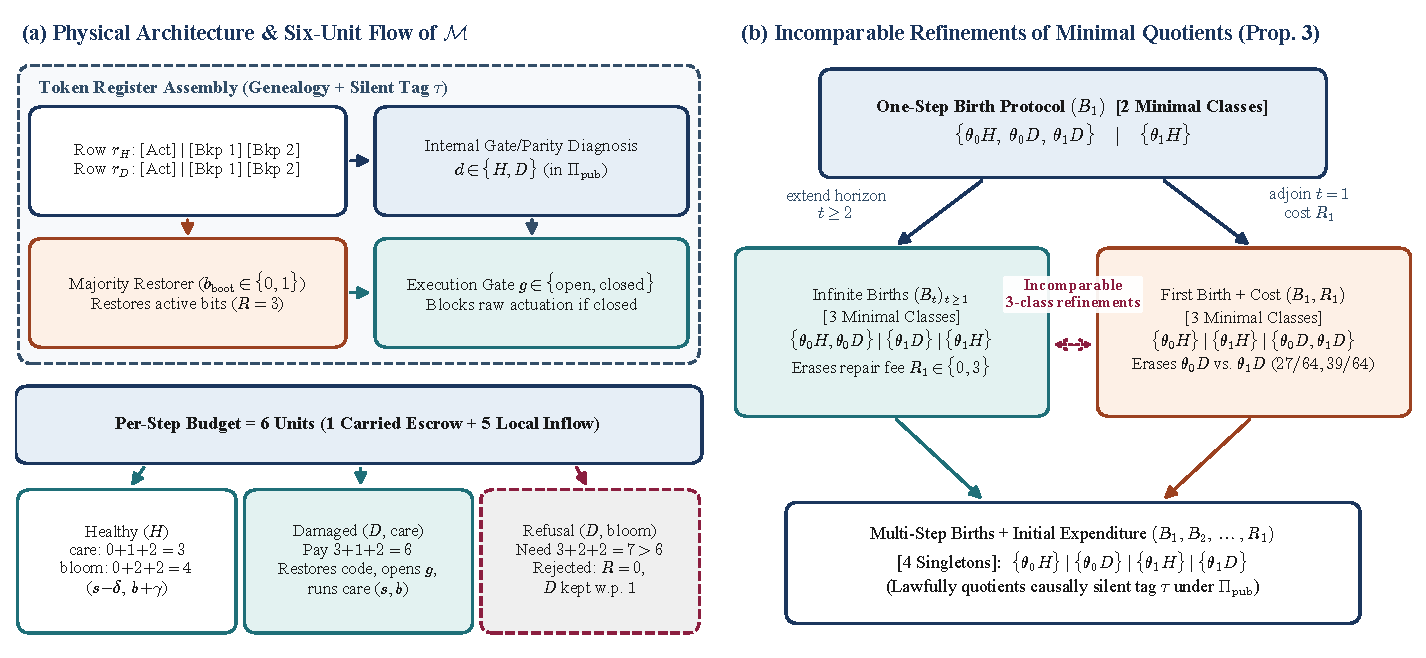
\includegraphics[width=0.98\linewidth,height=\textheight,keepaspectratio,alt={Physical
register architecture and predictive quotient lattice of the
regenerative process \textbackslash mathcal\{M\}. (a) Internal
three-cell instruction rows, parity/gate diagnostic, majority-vote
restorer, physical execution gate, and six-unit transaction paths. (b)
Diamond lattice of minimal predictive partitions across four observation
protocols (Proposition 3), showing two mutually incomparable three-class
refinements.}]{figures/fig1_architecture_and_lattice.pdf}
\caption{Physical register architecture and predictive quotient lattice
of the regenerative process \(\mathcal{M}\). (a) Internal three-cell
instruction rows, parity/gate diagnostic, majority-vote restorer,
physical execution gate, and six-unit transaction paths. (b) Diamond
lattice of minimal predictive partitions across four observation
protocols (Proposition 3), showing two mutually incomparable three-class
refinements.}
\end{figure}

\subsection{Lawful tag quotients versus von Neumann's
syntactic--constructor
gap}\label{lawful-tag-quotients-versus-von-neumanns-syntacticconstructor-gap}

\textbf{Proposition 4 (Silent-tag lumpability versus decoded-sequence
gate separation).} \emph{(a) Erasing silent tag \(\tau\) defines a
strong Markov lumpability \citep{burkeRosenblatt1958} commuting with
transitions, six-unit budgets, repair costs, genealogy, and expectations
across all \(\tau\)-blind policies lifted from the quotient (in
particular, across \(\Pi_{\mathrm{pub}}\)). (b) Projecting onto
majority-decoded code \(\theta \in \{\theta_0, \theta_1\}\) (even with
intact row parity) while erasing physical gate
\(g \in \{\mathrm{open}, \mathrm{closed}\}\) fails to determine raw
actuation: two intact \(\theta_1\) assemblies execute \texttt{bloom}
when \(g=\mathrm{open}\) (\(b+\gamma\)) but block raw actuation when
\(g=\mathrm{closed}\).}

Proposition 4 realises von Neumann's \citeyearpar{vonNeumann1966}
separation between passive syntactic tape and active gated constructor
\citep{rosen1991, deacon2011}. Biologically, this model is inspired by
\emph{Escherichia coli} methyl-directed DNA mismatch repair: biochemical
experiments establish that hemimethylated \texttt{GATC} strands guide
ATP-dependent \texttt{MutS–MutL–MutH} initiation coupled to active
replication forks \citep{auWelshModrich1992, hasanLeach2015}, motivating
the testable prediction (Section 6.2) that repaired and undamaged sister
lineages can share post-recovery division distributions while differing
in transient ATP depletion (\(R_1\)).

\section{Persistence, paid repair, and diachronic
bearers}\label{persistence-paid-repair-and-diachronic-bearers}

\subsection{Dynamical stability, servocontrol, paid repair, and
reciprocal
closure}\label{dynamical-stability-servocontrol-paid-repair-and-reciprocal-closure}

Universal loop or density signatures \citep{friston2013} conflate four
distinct regimes (Table 3). First, \emph{passive dynamical invariance}
(\(\dot{x} = -x\) on contractible \(\mathbb{R}^n\),
\(H_1(\mathbb{R}^n) = 0\)) yields compact \(\omega\)-limit sets
\(\omega(x_0) = \{0\}\) without cycles or repair. Second,
\emph{externally scaffolded servocontrol}
\citep{rosenblueth1943, conantAshby1970} regulates target variables via
fixed hardware it never regenerates. Third, \emph{paid endogenous repair
and constraint closure}
\citetext{\citealp[§§64--65]{kant1790}; \citealp{varela1974}; \citealp{maturanaVarela1980}; \citealp{weberVarela2002}; \citealp{rosen1991}; \citealp{kauffman1993}; \citealp{deacon2011}; \citealp{mossio2009}; \citealp{montevilMossio2015}}
use metabolic work to regenerate degrading enabling constraints
\citep{jonas1966, thompson2007}. Keeping our accounting exact,
\(\mathcal{M}\) is a \emph{minimal model of paid endogenous repair and
state-sensitive regulation}: on fast census steps
\(\tau_{\mathrm{step}}=1\), active rows and gate \(g\) degrade at rate
\(q\) and are rebuilt via \(b_{\mathrm{boot}}\) and backups, whereas
\(b_{\mathrm{boot}}=1\) is held fixed on a slower timescale
\(\tau_{\mathrm{boot}} \gg 1\). Full reciprocal Montévil--Mossio closure
requires an additional slow-timescale loop maintaining
\(b_{\mathrm{boot}}\) and backup templates themselves. Fourth,
\emph{adaptive viability}
\citep{aubinCellina1984, diPaolo2005, barandiaran2009, bich2024}
modulates modes relative to viability boundaries.

\Needspace{16\baselineskip}

{\def\LTcaptype{none} % do not increment counter
\begin{longtable}[]{@{}
  >{\raggedright\arraybackslash}p{(\linewidth - 6\tabcolsep) * \real{0.2500}}
  >{\raggedright\arraybackslash}p{(\linewidth - 6\tabcolsep) * \real{0.2500}}
  >{\raggedright\arraybackslash}p{(\linewidth - 6\tabcolsep) * \real{0.2500}}
  >{\raggedright\arraybackslash}p{(\linewidth - 6\tabcolsep) * \real{0.2500}}@{}}
\toprule\noalign{}
\begin{minipage}[b]{\linewidth}\raggedright
Persistence Regime
\end{minipage} & \begin{minipage}[b]{\linewidth}\raggedright
Sustaining Mechanism
\end{minipage} & \begin{minipage}[b]{\linewidth}\raggedright
Counterfactual Cut Signature
\end{minipage} & \begin{minipage}[b]{\linewidth}\raggedright
Paradigm Literature
\end{minipage} \\
\midrule\noalign{}
\endhead
\bottomrule\noalign{}
\endlastfoot
1. Passive invariance & Dissipative or conservative law (\(\dot{x}=-x\))
& Shifts orbit; zero constraint restoration & Topological dynamics \\
2. External servocontrol & Fixed feedback sensor--actuator & Regulates
state; zero hardware self-repair & \citet{rosenblueth1943};
\citet{conantAshby1970} \\
3. Paid repair \& closure & Work restores \(g\), active code; closure
loops \(b_{\mathrm{boot}}\) & Survives bounded damage; fails if
\(b_{\mathrm{boot}}\) cut & \citet{kant1790}; \citet{varela1974};
\citet{rosen1991}; \citet{montevilMossio2015} \\
4. Adaptive viability & History-sensitive policy in kernel \(K^\star\) &
Separates finite memory \(m\ge 1\) from \(m=0\) &
\citet{aubinCellina1984}; \citet{diPaolo2005}; \citet{bich2024} \\
\end{longtable}
}

Table 3. Four non-equivalent regimes of temporal persistence.

\subsection{Minimal cut-sets, finite-memory viability, and fixed-sample
limits}\label{minimal-cut-sets-finite-memory-viability-and-fixed-sample-limits}

Under monotone deletion failure on a downward-closed finite repertoire
\(\mathcal{I}\), destructive perturbations are uniquely represented by
the antichain of minimal cut-sets
\(\mathcal{V}_{\min}(\mathcal{C}, \mathcal{I})\) (\textbf{Proposition
5}, Appendix A.2)---isolating in \(\mathcal{M}\) bootstrap severance
(\(b_{\mathrm{boot}}=0\)), underfunding (\(2 < 3\)), and full three-cell
erasure \citep{coverThomas2006}, while failing under disinhibition.
Moreover (\textbf{Proposition 6}, Appendix A.2): \emph{(a)} on a
five-state system with maximal viable kernel
\(K^\star = \operatorname{gfp}(F_S) = S\) under pooled observation
\(h\), \emph{every} memoryless policy
\(\pi_0: \mathcal{O} \to \Delta(\mathcal{A})\) exits \(S\) in two steps
w.p. \(1/2\) whereas one-step memory
\(\pi_1: \mathcal{O}^2 \to \mathcal{A}\) maintains
\(\mathbb{P}_{\pi_1}(X_t \in K^\star\ \forall t \ge 0) = 1\) (Figure 2a)
\citep{kaelbling1998, papadimitriouTsitsiklis1987, sethTsakiris2018};
and \emph{(b)} for
\(Z_i \stackrel{\mathrm{i.i.d.}}{\sim} \mathrm{Bernoulli}(r)\), bounding
\(\mathbb{E}_r[\psi(Z_{1:n})] \le \alpha\) across all \(r \in (0,1]\)
forces \(\mathbb{E}_0[\psi] \le \alpha\) \citep{leCam1973, mayo2018}.

\subsection{Symmetrical fission as a stress test of relational
objecthood}\label{symmetrical-fission-as-a-stress-test-of-relational-objecthood}

Organisms persist through turnover while individuality splinters across
physiological, immunological, and Darwinian criteria
\citep{whitehead1929, clarke2010, godfreySmith2009, pradeu2012, maynardSmithSzathmary1995, dupreNicholson2018}.
Process \(\mathcal{M}\) separates parental retention from strict birth
despite identical post-step predictive classes \citep{wiggins2001}.
Symmetrical fission into two equally continuous, intervention-stable,
cost-accountable daughters \(y_1 \neq y_2\) \citep{parfit1984}
stress-tests Criteria (1)--(3) of Section 2.3: \emph{both} branches
satisfy all three criteria equally, yet transitivity blocks numerical
identity with both. Criteria (1)--(3) thus narrow candidates to cohesive
processes while leaving the residual choice among asymmetrical parent
indexing (as in \(\mathcal{M}\)), clonal termination into two new
tokens, and lineage tracking to explicit bearer indexing. Likewise, an
absorbing chain's \emph{quasi-stationary distribution}
\(\nu_{\mathrm{QSD}}\) differs from the \emph{Doob \(h\)-transformed}
survivor law \(\varpi(x) \propto \nu_{\mathrm{QSD}}(x)h(x)\)
\citep{doob1957, darrochSeneta1965, collet2013, cuciniello2026}.

\section{Optimisation, bearer divergence, and the grounds of
purpose}\label{optimisation-bearer-divergence-and-the-grounds-of-purpose}

\subsection{Evaluative underdetermination: reward shaping, gauge, and
bottleneck
rank}\label{evaluative-underdetermination-reward-shaping-gauge-and-bottleneck-rank}

Behavioural optimality never suffices for purpose: in inverse
reinforcement learning, observed policies fit an infinite cone of
rewards \citep[§3.1]{ngRussell2000}; in discounted dynamic programming
(\(\beta \in [0,1)\), or episodic settings with zero-potential proper
absorbing termination; \citet{blackwell1965}; \citet{puterman1994}),
potential-based reward shaping
\(r'(x,a,x') = r(x,a,x') + \beta\psi(x') - \psi(x)\) preserves optimal
policies \citep{ngHaradaRussell1999}; non-total multidimensional
preorders lack scalar utilities \citep{krantz1971}; and composite
resource--information scores \(J = R - \lambda I\)---comparable to
expected free energy \citep{parrPezzuloFriston2022} and distinct from
Tononi's \citeyearpar{tononi2004} \(\Phi^{\mathrm{IIT}}\)---admit exact
affine gauge freedom \(R' = R + \lambda\chi\), \(I' = I + \chi\).
Furthermore (\textbf{Proposition 7}, Appendix A.2), under healthy
\(\theta_0\) execution, the demographic-damage response map
\(\Psi(s,b,q) := (s, b, bq)\) has \(\det D\Psi = b > 0\) on the open
Table 1 domain: while this does not by itself refute scalar policy
objectives, it rules out \emph{losslessly reconstructing \((s,b,bq)\)
through any smooth two-variable \((R,I)\) bottleneck}.

\subsection{Full-policy growth ceiling versus autonomous hereditary
attainment}\label{full-policy-growth-ceiling-versus-autonomous-hereditary-attainment}

With per-token local six-unit sites, one-step output means are
\(k_c = s+b\) and \(k_b = s-\delta+b+\gamma\), giving hereditary rates
\(\lambda_0 = k_c\) and \(\lambda_1 = (1-q)k_b + q k_c\). Define the
admissible policy class \(\Pi_{\mathrm{pub}}\) explicitly: at each
census \(t\), \(\pi \in \Pi_{\mathrm{pub}}\) reads the public history
\(\mathcal{F}_t\) of living counts, per-token internal/public diagnoses
\(d_u \in \{H, D\}\), genealogical marks, and past expenditure receipts
(including \(\pi_{\mathrm{dorm}}\), which plays \texttt{care} on \(H\)
and \texttt{bloom} on \(D\)), using arbitrary joint randomisation across
living tokens while remaining blind to silent tags \(\tau\) and
contemporaneous/future actuation or damage noise.

\textbf{Theorem 1 (Full-policy growth ceiling versus autonomous
hereditary attainment).} \emph{For any strict parameters in Table 1 and
finite non-empty initial population \(P_0\), let
\(\rho_* := \max\{1, \lambda_0, \lambda_1\}\). (1) Across \textbf{all}
policies \(\pi \in \Pi_{\mathrm{pub}}\), there exists \(C > 0\) such
that \(\mathbb{E}_\pi[N_t] \le C \rho_*^t\) for all \(t \ge 0\), and a
stationary policy in \(\Pi_{\mathrm{pub}}\) attains
\(\Theta(\rho_*^t)\). (2) Under \textbf{autonomous multi-generational
execution of the fixed hereditary programme \(\theta_i\)}
(\(i \in \{0,1\}\)) from a single damaged founder \(\theta_i D\), paid
first-step repair (\(R_1=3\)), gate-mediated execution, and
\(\Theta(\rho_*^t)\) attainment hold jointly iff
\((\gamma \le \delta \land k_c \ge 1)\) for \(\theta_0\), and iff
\((\gamma \ge \delta \land \lambda_1 \ge 1)\) for \(\theta_1\).}

Separating the two quantifiers in Theorem 1 is essential: if a
controller in \(\Pi_{\mathrm{pub}}\) may \emph{abandon} hereditary
execution after \(t=1\), paid repair and \(\Theta(\rho_*^t)\) attainment
hold even in the subcritical regime! At
\((s,\delta,b,\gamma,q) = (1/2, 1/4, 1/4, 1/8, 1/3)\), \(k_c = 3/4\),
\(k_b = 5/8\), \(\lambda_1 = 2/3\), and \(\rho_* = 1\): neither
autonomous \(\theta_0\) nor autonomous \(\theta_1\) attains
\(\rho_*=1\), yet running \texttt{care} at \(t=1\) (\(R_1=3\), reopening
\(g\)) and switching to \(\pi_{\mathrm{dorm}}\) for \(t \ge 2\) retains
a damaged parent at \(t=2\) w.p. \(sq = 1/6\) (and leaves at least one
\(D\)-token w.p. \(17/72\)), yielding \(\Theta(1)\) via arrested
dormancy rather than active lineage reproduction.

Theorem 1 (Figure 2b) yields three further separations. First, the
subcritical floor \(\rho_* = 1\) (Regime I) arises from rejected damaged
\texttt{bloom}---analogous to dormant bacterial persisters surviving
harsh regimes where dividing lineages (\(\lambda_0,\lambda_1 < 1\))
decline. Second, in Regime III (\(\gamma > \delta, \lambda_1 \ge 1\)),
autonomous \texttt{bloom} maximises expected lineage growth while
\emph{reducing} parent survival (\(s-\delta < s\)), splitting organismal
persistence from lineage multiplication
\citep{okasha2006, godfreySmith2009} and \emph{differential retention}
from \emph{differential reproduction} \citep{garson2019}. Third, at
critical \((2/3, 1/8, 1/4, 1/4, 1/3)\), \(\lambda_1 = \rho_* = 1\) yet
\(\mathbb{E}_{\theta_1 D}[N_t] = 11/12 < 1\) for all \(t \ge 1\)
(\(k_c=11/12, k_b=25/24\)). At supercritical
\((3/4, 1/8, 3/8, 1/4, 1/3)\), independent healthy founders
\(\theta_1 H\) and \(\theta_0 H\) satisfy
\(\mathbb{P}(N_1^{(1)} = 0 \land N_1^{(0)} > 0) = 243/2048\), so the
higher-growth \(\theta_1\) lineage goes extinct at \(t=1\) while
\(\theta_0\) survives. Separately, defining the \(\theta_1\) population
share \(S_1 := N_1^{(1)}/(N_1^{(1)} + N_1^{(0)})\) (with \(S_1 := 0\)
when \(N_1^{(1)} = N_1^{(0)} = 0\)), the unconditional expectation is
\(\mathbb{E}[S_1] = 2095/4096\), the non-extinction-conditioned
expectation is
\(\mathbb{E}[S_1 \mid N_1^{(1)} + N_1^{(0)} > 0] = 2095/4006\), and the
ratio of expectations is
\(\mathbb{E}[N_1^{(1)}]/\mathbb{E}[N_1^{(1)}+N_1^{(0)}] = 10/19\)
\citep{price1970, athreyaNey1972}.

\begin{figure}
\centering
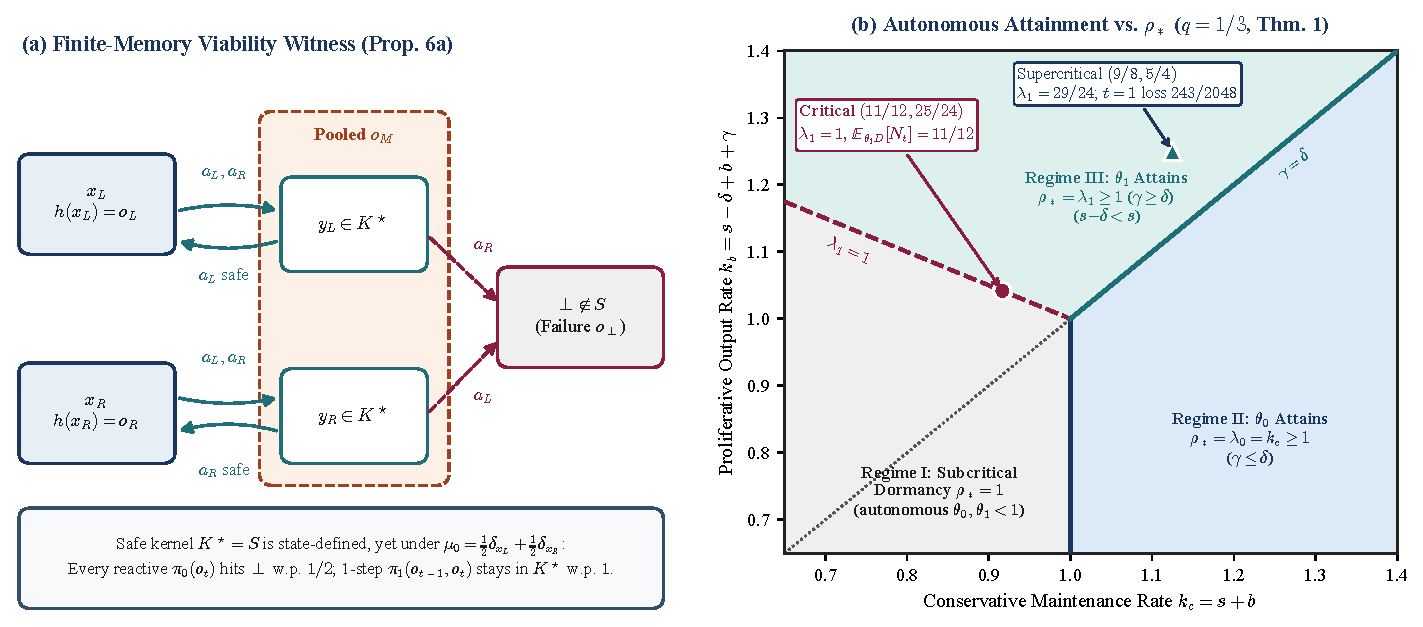
\includegraphics[width=0.98\linewidth,height=\textheight,keepaspectratio,alt={Finite-memory
viability separation and autonomous-versus-full-policy demographic phase
diagram. (a) Five-state partially observed viability witness
(Proposition 6a) where pooled observation o\_M forces every reactive
policy \textbackslash pi\_0(o\_t) into two-step failure w.p. 1/2 while
one-step memory \textbackslash pi\_1(o\_\{t-1\},o\_t) stays in
K\^{}\textbackslash star w.p. 1. (b) Exact (k\_c, k\_b) phase diagram at
q = 1/3 (Theorem 1), comparing the subcritical dormancy floor
(\textbackslash rho\_*=1) with autonomous hereditary attainment by
\textbackslash theta\_0 and \textbackslash theta\_1 and marking the
critical (11/12, 25/24) and supercritical (9/8, 5/4) rational
witnesses.}]{figures/fig2_memory_and_phase.pdf}
\caption{Finite-memory viability separation and
autonomous-versus-full-policy demographic phase diagram. (a) Five-state
partially observed viability witness (Proposition 6a) where pooled
observation \(o_M\) forces every reactive policy \(\pi_0(o_t)\) into
two-step failure w.p. \(1/2\) while one-step memory
\(\pi_1(o_{t-1},o_t)\) stays in \(K^\star\) w.p. \(1\). (b) Exact
\((k_c, k_b)\) phase diagram at \(q = 1/3\) (Theorem 1), comparing the
subcritical dormancy floor (\(\rho_*=1\)) with autonomous hereditary
attainment by \(\theta_0\) and \(\theta_1\) and marking the critical
\((11/12, 25/24)\) and supercritical \((9/8, 5/4)\) rational witnesses.}
\end{figure}

\subsection{Four stratified grounds of purpose and the normativity
challenge}\label{four-stratified-grounds-of-purpose-and-the-normativity-challenge}

Causal-role analysis \citep{cummins1975} lacks malfunction norms
\citep{davies2001}, selected-effects etiology
\citep{wright1973, millikan1984, neander1991, godfreySmith1994} misses
de novo regulation, and organisational accounts
\citep{mossio2009, bich2024} face Corti's \citeyearpar[§3]{corti2023}
and Bedau's \citeyearpar{bedau1992} challenge: why does existential
dependence support a functional \emph{ought}? Table 4 and Figure 3
stratify four non-interchangeable grounds:

\Needspace{16\baselineskip}

{\def\LTcaptype{none} % do not increment counter
\begin{longtable}[]{@{}
  >{\raggedright\arraybackslash}p{(\linewidth - 6\tabcolsep) * \real{0.2500}}
  >{\raggedright\arraybackslash}p{(\linewidth - 6\tabcolsep) * \real{0.2500}}
  >{\raggedright\arraybackslash}p{(\linewidth - 6\tabcolsep) * \real{0.2500}}
  >{\raggedright\arraybackslash}p{(\linewidth - 6\tabcolsep) * \real{0.2500}}@{}}
\toprule\noalign{}
\begin{minipage}[b]{\linewidth}\raggedright
Rung
\end{minipage} & \begin{minipage}[b]{\linewidth}\raggedright
Ground of Attribution
\end{minipage} & \begin{minipage}[b]{\linewidth}\raggedright
Bearer \& Required Evidence
\end{minipage} & \begin{minipage}[b]{\linewidth}\raggedright
Normative Scope \& Limit
\end{minipage} \\
\midrule\noalign{}
\endhead
\bottomrule\noalign{}
\endlastfoot
\textbf{1. Systemic role} & Constitutive decomposition
\citep{cummins1975, craver2007} & Part in capacity \(\Psi\); ablation
test & Explanatory relevance; \textbf{no} malfunction norm
\citep{davies2001} \\
\textbf{2. Regulatory repair} & Paid repair + control
\citep{nagel1977, mossio2009, diPaolo2005, bich2024} & Organism token;
gate/repair into \(K^\star\) & \emph{System-conditional functional
standard}; \textbf{not} categorical value \\
\textbf{3. Selective history} & Differential retention/reproduction
\citep{wright1973, millikan1984, garson2019} & Selected
lineage/repertoire; ancestral selection & \emph{Retrospective proper
function}; can \textbf{conflict} with Rung 2 \\
\textbf{4. Practical reason} & Reflective justification
\citep{korsgaard1996, scanlon1998, list2019} & Deliberative agent;
normative scrutiny & \emph{Justificatory ought}; \textbf{never} entailed
by Rungs 1--3 \citep{street2006} \\
\end{longtable}
}

Table 4. Four stratified grounds of functional and purposive
explanation.

\begin{enumerate}
\def\labelenumi{\arabic{enumi}.}
\tightlist
\item
  \textbf{Answering Corti at Rung 2 via conditional functional
  standards.} Pointing out that biology lacks moral obligations does not
  answer \citet{corti2023}; what answers Corti is showing what an
  \emph{objective system-conditional standard}---indexed to maintaining
  viable organisation \(K^\star\), without categorical value
  \citep{bedau1992} or evolutionary innovation claims
  \citep{cuciniello2026}---discriminates inside \(\mathcal{M}\)
  \citep{nagel1977, walsh2015}. Relative to maintaining executable
  integrity, \(\mathcal{M}\) sharply distinguishes \emph{(i)
  malfunction} (\(b_{\mathrm{boot}}=0\) or stuck \(g=\mathrm{closed}\)
  failing to restore execution under \texttt{care}), \emph{(ii)
  accidental side-effect survival} (subcritical rejected \texttt{bloom}
  preserving a damaged token as a budgetary by-product without restoring
  code or \(g\)), and \emph{(iii) costly normal operation} (damaged
  \texttt{care} paying \(R_1=3\) to restore active rows and execute).
\item
  \textbf{Prospective demographic advantage versus retrospective Rung 3
  function.} In a preset environment with \(\gamma > \delta\),
  \texttt{bloom} impairs Rung 2 parent survival (\(s-\delta < s\)) while
  raising \emph{prospective} lineage multiplication
  (\(\lambda_1 > \lambda_0\)). Respecting Table 4's evidential standard,
  \(\lambda_1 > \lambda_0\) alone is demographic propensity, \emph{not}
  yet a Rung 3 proper function: Rung 3 attribution additionally requires
  historical cohort-selection evidence that \(\theta_1\) persisted or
  spread \emph{because} of that proliferative effect.
\item
  \textbf{Scope of Rung 4.} Process \(\mathcal{M}\) contains no Rung 4
  witness; Rung 4 marks the boundary showing that Rungs 1--3 never by
  themselves entail practical endorsement
  \citep{korsgaard1996, street2006, list2019}.
\end{enumerate}

\begin{figure}
\centering
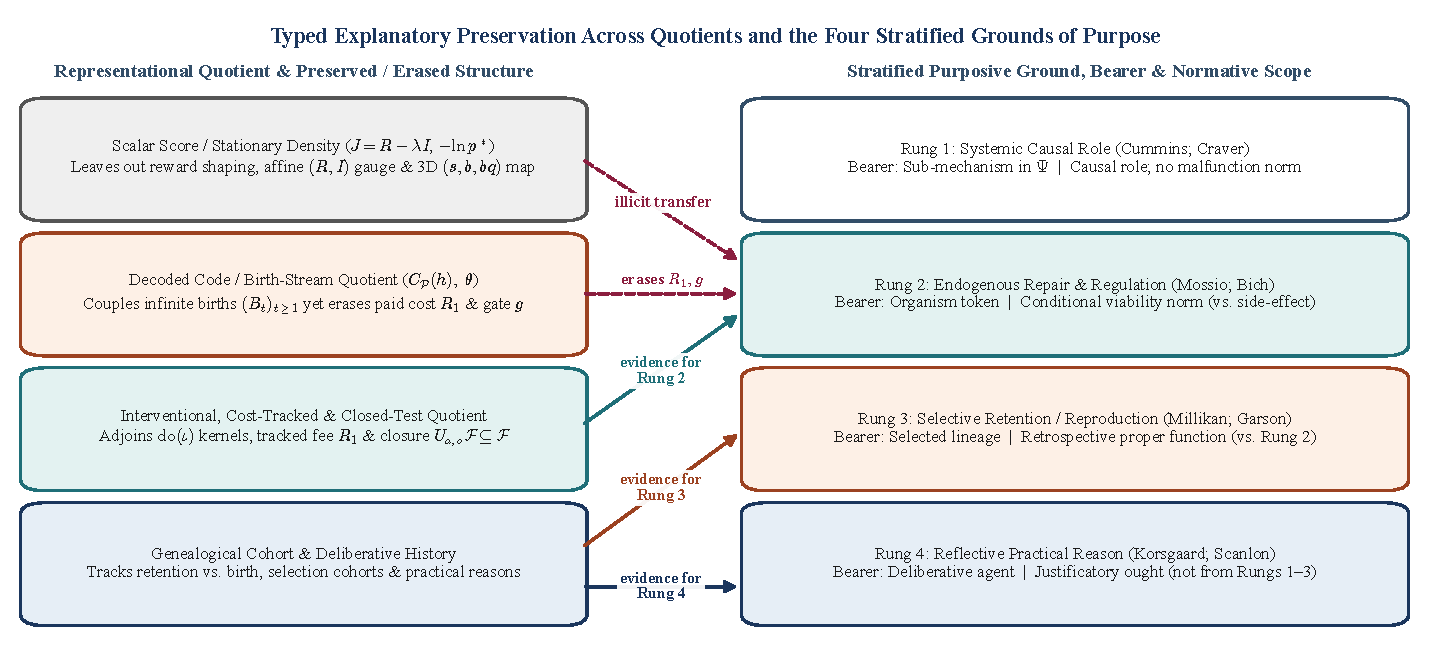
\includegraphics[width=0.98\linewidth,height=\textheight,keepaspectratio,alt={Summary
of typed explanatory preservation across representational quotients
(left) and its alignment with the four stratified grounds of functional
and purposive attribution (right), showing why interventional,
cost-tracked, and genealogical evidence are needed beyond output
quotients.}]{figures/fig3_preservation_and_rungs.pdf}
\caption{Summary of typed explanatory preservation across
representational quotients (left) and its alignment with the four
stratified grounds of functional and purposive attribution (right),
showing why interventional, cost-tracked, and genealogical evidence are
needed beyond output quotients.}
\end{figure}

\section{Competitor diagnostics, objections, and empirical
tests}\label{competitor-diagnostics-objections-and-empirical-tests}

\subsection{Diagnosing cross-protocol leaps in contemporary
programmes}\label{diagnosing-cross-protocol-leaps-in-contemporary-programmes}

\emph{(1) Active inference:} beyond the known distinction between
epistemic Pearl blankets and ontological Friston blankets
\citep{bruineberg2022, raja2021}, \(\mathcal{M}\) satisfies local sparse
mediation---internal rows \((r_H, r_D)\) act on births only via
diagnostic \(d\) and gate \(g\)
\citep{friston2013, parrPezzuloFriston2022}---yet boundary birth laws
\((B_t)_{t\ge 1}\) still erase paid repair \(R_1\), composite scores
retain affine gauge freedom \citep{biehl2021}, and parent survival
diverges from lineage growth, requiring Rung 2 hardware anchors
\citep{sethTsakiris2018}. \emph{(2) Computational mechanics:} minimal
\(\varepsilon\)-transducers
\citep{shaliziCrutchfield2001, barnettCrutchfield2015} and
macro-emergence \citep{hoel2013} are protocol-relative; Proposition 3
maps their cross-protocol transfer boundary. \emph{(3) Organisational
vs.~evolutionary teleology:} gate \(g\) captures state-sensitive
modulation \citep{bich2024} while genealogical records govern the
handoff from Rung 2 tokens to Rung 3 cohorts \citep{cuciniello2026}.

\subsection{Constructive unification and replies to four
objections}\label{constructive-unification-and-replies-to-four-objections}

Separate models \(\exists x\,R(x)\) and \(\exists y\,O(y)\) do not
entail \(\exists z\,[R(z)\land O(z)]\) when repair consumes half the
six-unit budget (\(3/6\)) and blocks damaged \texttt{bloom}
\citep{friedman1974, kitcher1989}; Theorem 1 establishes exact
constrained compatibility.

\begin{enumerate}
\def\labelenumi{\arabic{enumi}.}
\tightlist
\item
  \emph{Constructive empiricism suffices \citep{vanFraassen1980}.}
  Formal theorems never deductively compel realism. Our case is
  comparative \citep{hacking1983, woodward2003}: Proposition 3 shows
  that birth data \((B_t)_{t\ge 1}\) leave undamaged conservative
  execution \emph{(H0)} (\(R_1=0\)) and backup-plus-gate repair
  \emph{(H1)} (\(R_1=3\)) tied, whereas targeted ablations
  (\(b_{\mathrm{boot}}=0\), \(2\)-unit funding, gate inhibition) and
  calorimetry confirm \emph{(H1)}'s distinct counterfactual predictions
  \citep{mayo2018}.
\item
  \emph{Preservation is trivially analytic.} Fibre factorisation
  (\(F = \bar{F}\circ q\)) is analytic once \(F\) and \(q\) are fixed;
  the substantive work is proving \emph{which} compressions destroy
  \emph{which} invariants---including infinite-horizon cost erasure and
  incomparable protocol refinements (Proposition 3),
  sequence-versus-gate separation (Proposition 4b), finite-memory
  viability (Proposition 6a), and critical deficits (\(11/12 < 1\)).
\item
  \emph{Stipulated scaffolding falls short of full closure.} Exogenous
  energy inflow is shared by all living cells and does not render repair
  fictitious \citep{jonas1966, montevilMossio2015}. However, because
  \(b_{\mathrm{boot}}=1\) is fixed on the modelled horizon,
  \(\mathcal{M}\) establishes paid endogenous repair and state-sensitive
  regulation on the fast timescale, leaving slow-timescale regeneration
  of \(b_{\mathrm{boot}}\) (full reciprocal closure) and Rung 3
  selection as explicit additional conditions.
\item
  \emph{Empirical discrimination between rival mechanisms.} Passive
  birth equivalence does not imply that every birth-compatible model
  fails every intervention; rather, experiments adjudicate
  \emph{specified competing mechanisms} \citep{craver2007, mayo2018}. In
  synthetic microbial repair circuits
  \citep{auWelshModrich1992, hasanLeach2015}, four arms separate
  damage-free/cost-free \emph{(H0)} from ATP-paid template-and-gate
  repair \emph{(H1)}: \emph{(Arm 1)} matched post-recovery division
  distributions; \emph{(Arm 2)} transient single-cell ATP calorimetry
  isolating \(R_1\); \emph{(Arm 3)} replisome/transcriptional gate
  inhibition without sequence mutation; and \emph{(Arm 4)} microfluidic
  nutrient titration tracking mother-cell retention separately from
  daughter births.
\end{enumerate}

\section{Conclusion}\label{conclusion}

When two rival explanations share the exact same predictive law on an
output channel, what additional evidence warrants accepting one over the
other? Our results show that extending observations along different
coordinates produces mutually incomparable refinements, that autonomous
hereditary attainment of full-policy growth ceilings separates sharply
from plastic dormancy switching, and that parent survival can oppose
lineage multiplication. Calibrating relational objecthood and four-rung
bearer-indexed purpose strictly to these evidential boundaries preserves
explanatory unity without overclaiming beyond what mechanism, repair
budgets, and selection history warrant.

\appendix

\section{Self-contained proofs of Propositions 1--7 and Theorem
1}\label{self-contained-proofs-of-propositions-17-and-theorem-1}

\emph{Proof of Proposition 1.} Each countably generated
\(\Sigma_{\mathcal{Y}_i}\) is generated by a countable \(\pi\)-system
\(\mathcal{G}_i = \{G_{i,m}\}_{m\in\mathbb{N}}\) with
\(\mathcal{Y}_i \in \mathcal{G}_i\) \citep{kallenberg2021}. By
sufficiency of \(q\), for each \(i \in \mathcal{I}\) there exists
\(\widetilde{K}_i\) such that
\(N_i := \bigcup_{m\in\mathbb{N}} \{h \in \mathcal{H} : K_i(h, G_{i,m}) \neq \widetilde{K}_i(q(h), G_{i,m})\} \in \Sigma_{\mathcal{H}}\)
satisfies \(\mu(N_i) = 0\); by Dynkin's \(\pi\)-\(\lambda\) theorem,
\(K_i(h, \cdot) = \widetilde{K}_i(q(h), \cdot)\) for all
\(h \notin N_i\). Defining
\(\psi(z) := (\widetilde{K}_i(z, \cdot))_{i\in\mathcal{I}}\) and
\(N := \bigcup_{i\in\mathcal{I}} N_i\), countability of \(\mathcal{I}\)
gives \(\mu(N) \le \sum_{i\in\mathcal{I}} \mu(N_i) = 0\), with
\(C_{\mathcal{P}}(h) = \psi(q(h))\) on \(\mathcal{H}\setminus N\).
\(\square\)

\emph{Proof of Proposition 2.} Let
\(b'_{a,o}(x') = \sum_{x} b(x) T(x'\mid x,a) O(o\mid a,x')\); then
\(\langle b'_{a,o}, f\rangle = \langle b, U_{a,o}f\rangle\) and
\(p(o\mid b,a) = \langle b, U_{a,o}\mathbf{1}\rangle\).
(\emph{Sufficiency}) If \(U_{a,o}\mathcal{F} \subseteq \mathcal{F}\) and
\(b \equiv_{\mathcal{F}} \tilde{b}\), then
\(U_{a,o}\mathbf{1} \in \mathcal{F}\) gives
\(p(o\mid b,a) = p(o\mid \tilde{b},a)\), and for \(p(o\mid b,a) > 0\),
\(\langle \mathrm{Bayes}(b,a,o), f\rangle = \langle b, U_{a,o}f\rangle / p(o\mid b,a) = \langle \mathrm{Bayes}(\tilde{b},a,o), f\rangle\)
(\(\forall f \in \mathcal{F}\)). (\emph{Necessity}) Assume (i)--(ii) on
\(\Delta(\mathcal{X})\). For \(v \in \mathcal{F}^\perp\),
\(\langle v, \mathbf{1}\rangle = 0\). Perturbing
\(b^\circ(x) = 1/|\mathcal{X}|\) to
\(\tilde{b} = b^\circ + \varepsilon v \in \Delta(\mathcal{X})\), (i)
forces \(\langle v, U_{a,o}\mathbf{1}\rangle = 0\)
(\(\forall v \in \mathcal{F}^\perp\)), so
\(U_{a,o}\mathbf{1} \in \mathcal{F}\). For \(f \in \mathcal{F}\), if
\(p_0 := p(o\mid b^\circ, a) = 0\), positivity of \(b^\circ\) gives
\(U_{a,o}\mathbf{1} \equiv 0\) and \(U_{a,o}f = 0 \in \mathcal{F}\); if
\(p_0 > 0\), (ii) gives \(\langle v, U_{a,o}f\rangle / p_0 = 0\)
(\(\forall v \in \mathcal{F}^\perp\)), so \(U_{a,o}f \in \mathcal{F}\).
\(\square\)

\emph{Proofs of Propositions 5, 6, and 7.} \emph{(Prop. 5)} Upward
closure follows from monotonicity; downward closure of finite
\(\mathcal{I}\) yields a minimum-cardinality \(M \subseteq D\) in
\(\mathcal{F}\), lying in the unique antichain \(\mathcal{V}_{\min}\).
\emph{(Prop. 6a)} On \(\mathcal{X} = \{x_L, x_R, y_L, y_R, \bot\}\),
\(S = \{x_L, x_R, y_L, y_R\}\), \(\mathcal{A} = \{a_L, a_R\}\), set
\(h(x_L)=o_L\), \(h(x_R)=o_R\), \(h(y_L)=h(y_R)=o_M\),
\(h(\bot)=o_\bot\), with \(x_L \to y_L\), \(x_R \to y_R\) under
\(\{a_L,a_R\}\); \(y_L \xrightarrow{a_L} x_L\),
\(y_L \xrightarrow{a_R} \bot\); \(y_R \xrightarrow{a_R} x_R\),
\(y_R \xrightarrow{a_L} \bot\); and \(\bot\) absorbing
(\(K^\star = S\)). Under
\(\mu_0 = \frac{1}{2}\delta_{x_L} + \frac{1}{2}\delta_{x_R}\), any
\(\pi_0(a_L \mid o_M) = p\) gives
\(\mathbb{P}_{\pi_0}(X_2 = \bot) = \frac{1}{2}(1-p) + \frac{1}{2}p = \frac{1}{2}\),
whereas \(\pi_1(o_L,o_M)=a_L\), \(\pi_1(o_R,o_M)=a_R\) keeps
\(X_t \in K^\star\) w.p. \(1\). \emph{(Prop. 6b)}
\(|g(0) - g(\varepsilon)| \le d_{\mathrm{TV}}(\mathrm{Bern}(0)^{\otimes n}, \mathrm{Bern}(\varepsilon)^{\otimes n}) = 1 - (1-\varepsilon)^n \le n\varepsilon\),
so \(\sup_{r>0} g(r) \le \alpha \implies g(0) \le \alpha\). \emph{(Prop.
7)}
\(\det D\Psi(s,b,q) = \det \bigl(\begin{smallmatrix}1&0&0\\0&1&0\\0&q&b\end{smallmatrix}\bigr) = b > 0\),
contradicting \(\operatorname{rank}(Dg \cdot Df) \le 2\). \(\square\)

\emph{Proofs of Propositions 3 and 4.} Across any strict Table 1
parameter vector (using only \(\gamma > 0\), \(s+b > 0\), \(1-q > 0\)):
at \(t=1\), \(\theta_0 H\) (\(R_1=0\)) and repaired
\(\theta_0 D, \theta_1 D\) (\(R_1=3\)) run \texttt{care}
(\(B_1 \sim \mathrm{Bern}(b)\)), while \(\theta_1 H\) (\(R_1=0\)) runs
\texttt{bloom} (\(B_1 \sim \mathrm{Bern}(b+\gamma)\)), giving two
\(B_1\)-classes and three \((B_1,R_1)\)-classes. After \(t=1\),
\(\theta_0 H\) and \(\theta_0 D\) leave identically distributed
\(\theta_0\)-populations
\((I_{\mathrm{ret}}, B_1) \sim \mathrm{Bern}(s)\otimes\mathrm{Bern}(b)\)
with independent damage \(q\), coupling \((B_t)_{t\ge 1}\) identically.
At \(t=2\), \(\mathbb{E}[N_1] = s+b\) for both \(\theta_0 D\) and
\(\theta_1 D\), giving \(\mathbb{E}_{\theta_0 D}[B_2] = (s+b)b\) versus
\(\mathbb{E}_{\theta_1 D}[B_2] = (s+b)[(1-q)(b+\gamma)+qb]\); their
difference \((s+b)(1-q)\gamma > 0\) yields three
\((B_t)_{t\ge 1}\)-classes (\(27/64\) vs.~\(39/64\) at
\((3/4,1/8,3/8,1/4,1/3)\)), refined to four singletons on
\((B_{1:T}, R_1)\). For Prop. 4, \(\tau\) enters no kernel or cost rule,
commuting with all \(\tau\)-blind policies (including
\(\Pi_{\mathrm{pub}}\)), whereas intact \(\theta_1\)-decoded assemblies
with \(g=\mathrm{open}\) versus \(g=\mathrm{closed}\) diverge under raw
actuation. \(\square\)

\emph{Proof of Theorem 1.} \textbf{(1)} Set \(v(H) := \max\{k_c, k_b\}\)
and \(v(D) := k_c\) (\(0 < k_c \le v(x) \le v_{\max}\)). Any executed
step with mean output \(k \in \{k_c, k_b\}\) has expected post-damage
potential \((L_a v)(x) = k[(1-q)v(H) + q v(D)]\). If
\(\gamma \le \delta\) (\(k_b \le k_c\)), \(v \equiv k_c\),
\(\rho_* = \max\{1, k_c\}\), and
\((L_a v)(x) \le \max\{k_c^2, k_b k_c, k_c, 0\} \le \rho_* v(x)\). If
\(\gamma > \delta\) (\(k_b > k_c\)), \(v(H)=k_b\), \(v(D)=k_c\),
\(\lambda_1 = (1-q)k_b + q k_c > \lambda_0\), and
\(\rho_* = \max\{1, \lambda_1\}\):
\((L_{\mathrm{bloom}}v)(H) = k_b \lambda_1 = \lambda_1 v(H)\),
\((L_{\mathrm{care}}v)(H) = k_c \lambda_1 < \lambda_1 v(H)\),
\((L_{\mathrm{care}}v)(D) = k_c \lambda_1 = \lambda_1 v(D)\), and
rejected \((D,\mathrm{bloom})\) yields \(v(D) \le \rho_* v(D)\). Summing
\(V(P_t) = \sum_{u\in P_t} v(x_u)\) under \(\pi \in \Pi_{\mathrm{pub}}\)
gives
\(\mathbb{E}_\pi[V(P_{t+1})\mid \mathcal{F}_t] \le \rho_* V(P_t)\), so
\(\mathbb{E}_\pi[N_t] \le (v_{\max}|P_0|/k_c)\rho_*^t\). Tightness holds
via \(\pi_{\mathrm{dorm}} \in \Pi_{\mathrm{pub}}\) (\texttt{care} on
\(H\), \texttt{bloom} on \(D\)) when \(\rho_*=1\)
(\(\mathbb{E}_{\pi_{\mathrm{dorm}}}[N_t] \ge \min\{1, sq\}\)),
stationary \(\theta_0\) when \(\rho_*=\lambda_0\), and stationary
\(\theta_1\) when \(\rho_*=\lambda_1\)
(\(\mathbb{E}_{\theta_1}[V(P_t)] = V(P_0)\lambda_1^t\)). \textbf{(2)}
Under autonomous execution from damaged founders,
\(\mathbb{E}_{\theta_0 D}[N_t] = k_c^t\)
(\(\Theta(\rho_*^t) \iff \gamma\le\delta \land k_c\ge 1\)) and
\(\mathbb{E}_{\theta_1 D}[N_t] = k_c \lambda_1^{t-1}\) for \(t \ge 1\)
(\(\Theta(\rho_*^t) \iff \gamma\ge\delta \land \lambda_1\ge 1\)). Under
switching in \(\Pi_{\mathrm{pub}}\) at \((1/2,1/4,1/4,1/8,1/3)\)
(\(k_c=3/4, k_b=5/8, \lambda_1=2/3, \rho_*=1\)), running \texttt{care}
at \(t=1\) (\(R_1=3\)) and \(\pi_{\mathrm{dorm}}\) for \(t\ge 2\)
retains a damaged parent at \(t=2\) w.p. \(sq = 1/6\) (at least one
\(D\)-token w.p. \(17/72\)), giving
\(\mathbb{E}[N_t] \ge 1/6 = \Theta(1)\). At \((2/3,1/8,1/4,1/4,1/3)\),
\(k_c=11/12, k_b=25/24, \lambda_1=1\), so
\(\mathbb{E}_{\theta_1 D}[N_t] = 11/12\). At \((3/4,1/8,3/8,1/4,1/3)\),
\(N_1^{(1)} \sim (9/64, 30/64, 25/64)\) and
\(N_1^{(0)} \sim (5/32, 18/32, 9/32)\), giving
\(\mathbb{P}(N_1^{(1)}=0 \land N_1^{(0)}>0) = \frac{9}{64}\cdot\frac{27}{32} = \frac{243}{2048}\),
\(\mathbb{E}[N_1^{(1)}]/\mathbb{E}[N_1^{(1)}+N_1^{(0)}] = \frac{5/4}{19/8} = \frac{10}{19}\),
\(\mathbb{E}[S_1] = \frac{30}{64}\cdot\frac{17}{32} + \frac{25}{64}\cdot\frac{43}{64} = \frac{2095}{4096}\),
and
\(\mathbb{E}[S_1 \mid N_1^{(1)}+N_1^{(0)} > 0] = \frac{2095}{4006}\).
\(\square\)

\clearpage
\begingroup
\onehalfspacing
\setlength{\bibsep}{4pt}
\bibliographystyle{plainnat}
\bibliography{references}
\endgroup
\end{document}
